\documentclass{article}

% Packages
\usepackage{amsmath}
\usepackage{graphicx}
\usepackage[round]{natbib}
\usepackage{subcaption}
\usepackage{todonotes}

% Document metadata
\title{Untitled EnKF paper}
\author{Keiran Suchak}

\begin{document}

\maketitle{}

\begin{abstract}
    Write abstract here.
\end{abstract}

% *********************************************************************************
% *********************************************************************************
% *********************************************************************************
\section{Introduction}\label{sec:intro}

Contents:
\begin{itemize}
    \item Provide context and motivation for investigation.
    \item Outline aims and objectives.
\end{itemize}

Main aim: show that an Ensemble Kalman Filter (EnKF) can improve the accuracy with which an agent-based model simulates a system of pedestrians.

Points of distinction to highlight:
\begin{itemize}
    \item Defining an approach for defining whether an agent is active or
        inactive in an ensemble of models.
    \item Comparing error in ensemble mean with mean of errors of
        ensemble-member models.
    \item Explaining the importance of an appropriate summary statistic
        (median instead of mean) when calculating the average error over
        time.
    \item Explaining the importance of considering time-steps when a
        sufficient number of filters are still running when collecting
        summary statistics of multiple filter runs.
    \item Using EnKF to improve the accuracy with which an ABM simulates a
        pedestrian system.
\end{itemize}

Other things to mention in the introduction:
\begin{itemize}
  \item Pseudo-truth data. ``The purpose of the base model for these experiments is simply to provide a state against which to compare the performance of filters.''
  \item Broad overview of the experimental approach (how do the experiments show that the EnKF is/isn't working?)
\end{itemize}





% *********************************************************************************
% *********************************************************************************
% *********************************************************************************
\section{Background}\label{sec:background}

\begin{itemize}
    \item Discuss previous relevant work:
    \begin{itemize}
        \item \citet{ward2016dynamic}
        \item \citet{malleson2020simulating}
        \item \citet{clay2020towards}
    \end{itemize}
\end{itemize}


% *********************************************************************************
% *********************************************************************************
% *********************************************************************************
\section{Methods}\label{sec:methods}

\subsection{Model}\label{sub:methods:model}

Explain about \texttt{StationSim\_GCS}.

Things to note:
\begin{itemize}
  \item What an `active' agent is
\end{itemize}

\subsection{Ensemble Kalman Filter}\label{sub:methods:enkf}

\begin{itemize}
    \item Explain about the Ensemble Kalman Filter~\citep{evensen2003ensemble},
        which is based on the Kalman Filter~\citep{kalman1960new}.
    \item Point to previous experiments in the thesis. E.g. ``Results: The data assimilation scheme was tested for a range of different filter
parameter values, and it was found that improvements in filter performance
resulted from increases in the ensemble size, reductions in the standard
deviation of the observation error and reductions in the number of time-steps
between successive attempts to assimilate observational data into the system.'' (p113)
\end{itemize}



% *********************************************************************************
% *********************************************************************************
% *********************************************************************************
\section{Experiments}\label{sec:exp}

The experiments, outlined visually in Figure~\ref{fig:exp}, aim to demonstrate that the EnFK can improve the accuracy of a pedestrian system in comparison to a baseline scenario with no data assimilation. In order to better understand the impact of data assimilation on an agent-based model, rather assess the realism of the model itself, we use the ``identical twin'' approach \citet{lueck_who_2019}. In this approach, a `Base Model' is used. A Base Model is an instance of    \texttt{StationSim\_GCS} that is used to generate `pseudo-true' data that are taken as the real-world observations in the experiments (in lieu of data from a real crowd).

%The experiments run for this chapter can be found in the notebooks found in \texttt{Projects/ABM\_DA/experiments/enkf\_experiments/results\_2/notebooks/} in the \href{https://zenodo.org/record/6469804}{dust repository archive}}.

\begin{figure}[htbp]
    \centering
    \begin{subfigure}[htb]{0.80\textwidth}
        \centering
        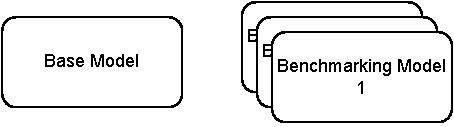
\includegraphics[width=\textwidth ]{figures/exp_1}
        \caption{Experiment 1: Benchmarking}\label{fig:exp:exp_1}
    \end{subfigure}

    \vspace{2em}
    
    \begin{subfigure}[htb]{0.80\textwidth}
        \centering
        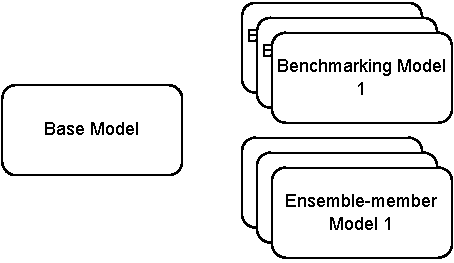
\includegraphics[width=\textwidth]{figures/exp_2}
        \caption{Experiment 2: Exploring Ensemble-Member Models}\label{fig:exp:exp_2}
    \end{subfigure}
    
    \vspace{2em}
    
    \begin{subfigure}[htb]{0.80\textwidth}
        \centering
        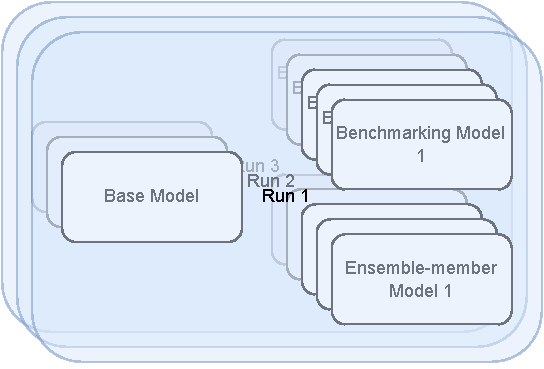
\includegraphics[width=\textwidth]{figures/exp_3}
        \caption{Experiment 3: Implementing the Ensemble Kalman
        Filter}\label{fig:exp:exp_3}
    \end{subfigure}
    \caption{Graphical outline of the three experiments. Note that the 'base model' is use to generate pseudo-true observation data }\label{fig:exp}
\end{figure}

The initial experiment, (`benchmarking', Figure~\ref{fig:exp:exp_1}) seeks to establish a benchmark against which to compare subsequent implementations of the EnKF. 
This is achieved by running an ensemble of models, each initialised as duplicates of a base model which is used to generate pseudo-truth values for the system state.

The second experiment (Figure~\ref{fig:exp:exp_2}) seeks to XXXX\todo[]{Keiran what is the higher-level purpose of this experiment?}. It does this by exploring the variation in the accuracy of individual ensemble members. 
This is achieved by running a single EnKF which maintains a benchmarking ensemble of models, providing a baseline against which to compare results, along with and ensemble of models that are periodically updated by the EnKF assimilation process. In such a situation, we are able to compare the average error per agent in each of the ensemble member models at each assimilation time-step.

The final experiment (Figure~\ref{fig:exp:exp_3}) takes this exploration a step further by seeking to capture the variation in error at an ensemble level.\todo{Again, why?} This involves running a collection of EnKFs for the same set of model and filter parameters, and in each case gathering data regarding the variation in the error in the ensemble mean state over time, comparing this with
the variation in the corresponding collection of benchmark errors.

In all experiments the following approach is taken:
\begin{enumerate}
    \item Create an instance of the model to be considered the base model which
        provides pseudo-truth states of the pedestrian system.
    \item Create an ensemble of 100 models, each of which is a copy of the base
        model; this means that each of the duplicates in the ensemble contain
        the same information regarding which exits each of the agents will enter
        and exit through, as well as at what time they will be activated within
        the model. These models, however, are liable to diverge from the base
        model due to the collisions that occur between pedestrian agents.
    \item Iterate each of the base model and the ensemble of models forward for
        each time-step. At each time-step, calculate average model state for
        each agent in the system population, and calculate the average error per
        agent between this average model state and the pseudo-truth state
        generated from the base model for this time-step.
\end{enumerate}


\subsection{Measuring Error}\label{sec:error}

\begin{itemize}
    \item Talk about measures used when running experiments with multiple EnKFs
        to ensure that outliers don't skew results:
    \begin{itemize}
        \item Median instead of mean error.
        \item Only considering time-steps when a sufficient number of models are
            active.
    \end{itemize}
\end{itemize}

\subsection{Active and inactive agents}

As this following sections will discuss, error is calculated by comparing the positions of agents in the simulation with the positions of corresponding agents in the base model (i.e. the pseudo-truth data, discussed in \ref{sec:exp}). To do this, it is necessary to consider whether an agent is `active' 
or `inactive' as once an agent has left the simulation they should not be included in an error calculation. However, an agent might be active in the base (pseudo-truth) model and inactive in some or all of the EnKF ensemble members, or vice versa.  
Here we assume that an agent is active only while it is active in the EnKF ensemble  because in a real situation we would not necessarily have access to the true positions of the individuals in the crowd, so could only assess an agent's status from the information available in the ensemble of models. Hence an agent is considered active if its most common (i.e. modal) status across the ensemble is active.

\subsubsection{Agent-level error}

Error at the level of the individual agents is quantified by calculating the distance between the position of an agent estimated by the ensemble of models in te EnKF and the position of the corresponding agent in the base model, $d_i$:
\begin{equation}
    d_i = 
    \begin{cases}
        | \hat{\mathbf{x}}_i - \mathbf{x}_i | & \text{if $i$th agent is
        active;}\\
        0 & \text{otherwise,}
    \end{cases}
\end{equation}
where $\hat{\mathbf{x}}_i$ is the $x$-$y$ position of the $i$th agent estimated by the ensemble of models and $\mathbf{x}_i$ is the $x$-$y$ position of the $i$th agent in the base model. The distance between the $\hat{\mathbf{x}}_i$ and $\mathbf{x}_i$ agent is calculated using the Euclidean distance.

\subsubsection{Model-level error}

To calculate the error across the whole system, we calculate the average distance over all active agents in the system, $\bar{d}$:
\begin{equation}
    \bar{d} = \frac{1}{N} \sum_{i=1}^{N} d_i,
\end{equation}
where $N$ is the number of \emph{active} agents. This average distance, $\bar{d}$, can then be used to measure the error in an ensemble of models given the ensemble mean state for a given time-step and the base model state at the same time-step. 
In this way, we create a base model which is used to generate a ground truth and an ensemble of models from which we can obtain the average behaviour behaviour by averaging across the ensemble. 
The accuracy with which this average behaviour simulates the ground truth generated by the base model is assessed by considering the error between the base model and the average of the ensemble.



\subsection{Experiment 1: Benchmarking}\label{sub:exp:bench}

The initial experiment to be performed is to develop a model baseline, establishing the effectiveness of \texttt{StationSim\_GCS} in modelling a system in the absence of any information whilst running. 

This is applied to ensembles with increasing population sizes (as per Table~\ref{tab:gcs_baseline_params}) to explore how this behaviour varies with population size.

\begin{table}
    \centering
    \begin{tabular}{@{}lc@{}}
        \toprule
        Parameter           & Value \\ \midrule
        Population size     & $[10, 20, 50, 100 ]$   \\
        Ensemble size       & 100   \\
        Number of entrances & 11    \\
        Number of exits     & 11    \\
        Environment height  & 700   \\
        Environment width   & 740   \\ \bottomrule
    \end{tabular}\caption{Table of model parameters used for estimating the
    baseline level of error.}\label{tab:gcs_baseline_params}
\end{table}

% DESCRIPTION OF EXPECTATIONS OF THE RESULTS:
%Having followed these steps to collect data regarding how the error of an
%ensemble of models varies over time without any observations being assimilated,
%we can then plot this as a time-series.
%We expect that, whilst the initial error in the benchmarking ensemble will be
%low by virtue of the ensemble-member models being copies of the base model, this
%error will grow rapidly as agents enter the environment.
%As a growing number of agents are present in the system, the chance of
%inter-agent interactions occurring increases, and as such so does the chance
%that the ensemble mean state diverge from the base model state.
%With no observations being assimilated into the ensemble of models, these
%divergences go uncorrected.
%Consequently, we expect to observe an increase in the benchmarking error.
%As the ensemble of models near completion, i.e. a state where all of the agents
%in the ensemble member models have finished their journeys and are deactivated,
%we expect to see the average error per agent to fall, nearing $0$.
%As with the expectation that the initial average error per agent is low, this
%would be a consequence of each of the ensemble member models being a copy of the
%base model, and therefore each of the agents in these member models having the
%same target destination as the corresponding agent in the base model.


\subsection{Experiment 2: Exploring Ensemble Members}

\todo[inline]{Better word than 'exploring' above? Something more specific?}


\subsection{Experiment 3: Assesing the EnKF}


% *********************************************************************************
% *********************************************************************************
% *********************************************************************************
\section{Results}\label{sec:results}

\subsection{Benchmarking}\label{sub:results:bench}


% *********************************************************************************
% *********************************************************************************
% *********************************************************************************
\section{Conclusion}\label{sec:conc}

\bibliographystyle{unsrtnat}
\bibliography{references}

\end{document}
